\documentclass[11pt]{article}

\usepackage[top=20mm, bottom=20mm, inner=25mm, outer=25mm]{geometry}
\usepackage[title, toc]{appendix}
\usepackage[font=scriptsize, labelfont=it, textfont=it]{caption}
\usepackage{graphicx}
\usepackage{setspace}
\usepackage{enumitem}
\usepackage[parfill]{parskip}
\usepackage{nameref}
\usepackage{multirow}
\usepackage{outlines}
\usepackage{hyperref}

\setlength{\parindent}{0pt}

\begin{document}

%%%%%%%%%%%%%%%%%%%%%%%%%%%%%%%%%%%%%%%%%%%%%%%%%%%%%%%%%%%%%%%%%%%%%%%%%%%%%%%%

\onehalfspacing
\begin{titlepage}
    \begin{center}
        \Huge
        \textbf{UNSW} \\

        \vspace{5mm}

        
\includegraphics[height=4cm]{unsw-logo.jpg}

        \vspace{5mm}

        \Large
        Faculty of Engineering \\
        School of Computer Science \& Engineering \\

        \vspace{10mm}

        \textbf{COMP3431} \\
        Robot Software Architectures \\

        \vspace{15mm}

        \LARGE
        \textbf{Project 2 Individual Report} \\
        
        \Large
        Group: Bob Ros

        \vspace{15mm}

        \Large
        Course Coordinator: Claude Sammut\\
        Due Date: 29/11/2020 \\

        \vfill
        \rule{\linewidth}{0.5pt} \\

        \Large
        Dan Nguyen \\

        \large
        z5206032 \\

    \end{center}
\end{titlepage}

\pagenumbering{roman}

%%%%%%%%%%%%%%%%%%%%%%%%%%%%%%%%%%%%%%%%%%%%%%%%%%%%%%%%%%%%%%%%%%%%%%%%%%%%%%%%

\begin{abstract}
    Autonomous driving is widely considered to be the next step in revolutionising the automobile industry in the foreseeable future. However this technology is far from mature and requires improvements in safety and reliability before autonomous driving can be commercialised. The purpose of this research paper is to explore a simple robotic software architecture (in accordance with the learning objectives of COMP3431) to handle the autonomous driving of a TurtleBot3 Waffle Pi in real-time, sparse-road, constant-illumination conditions using a Raspberry Pi camera sensor and OpenCV2 library. The autonomous driving system was adequate in the project demonstration for COMP3431 and its performance is evaluated with some suggestions for improvements.
\end{abstract}
\pagebreak

%%%%%%%%%%%%%%%%%%%%%%%%%%%%%%%%%%%%%%%%%%%%%%%%%%%%%%%%%%%%%%%%%%%%%%%%%%%%%%%%

\tableofcontents
\vspace{1cm}
\listoffigures
\vspace{1cm}
\pagebreak

\pagenumbering{arabic}

%%%%%%%%%%%%%%%%%%%%%%%%%%%%%%%%%%%%%%%%%%%%%%%%%%%%%%%%%%%%%%%%%%%%%%%%%%%%%%%%

\section{Introduction}
\label{sec:intro}

    Autonomous driving is the ability for a vehicle to drive itself with minimal or no human interaction, and is considered to be the next leap in innovation for the automobile industry. Research into this technology is pushed by its benefits of increased traffic efficiency, increase in quality of life, and potential reduction of traffic accidents. For autonomous driving to be feasible, a software architecture must be described. In the most simplistic form, sensors are required for the vehicle to perceive its environment, the sensor data processed then a decision must be made to actuate the vehicle \cite{autonomous_driving_changes_future}. However in reality, autonomous driving software architectures are complex with various types of sensors and detailed vehicle control planning. This has applied limitations on the technology as it is not mature for commercialisation where accuracy, reliability, speed, and safety are the limiting key factors.
    
    The development of autonomous driving requires the knowledge of robotic software architectures where this report explores the use of a simple 2-layered robotic software architecture and discusses the appropriateness and fundamental layers of this stack in achieving autonomous driving on the Turtlebot3 Waffle Pi in a controlled environment.

\section{Environment}
\label{sec:environment}

    The environment is shown in Figure \ref{fig:environment} below.

    \begin{figure}[h!]
        \centering
        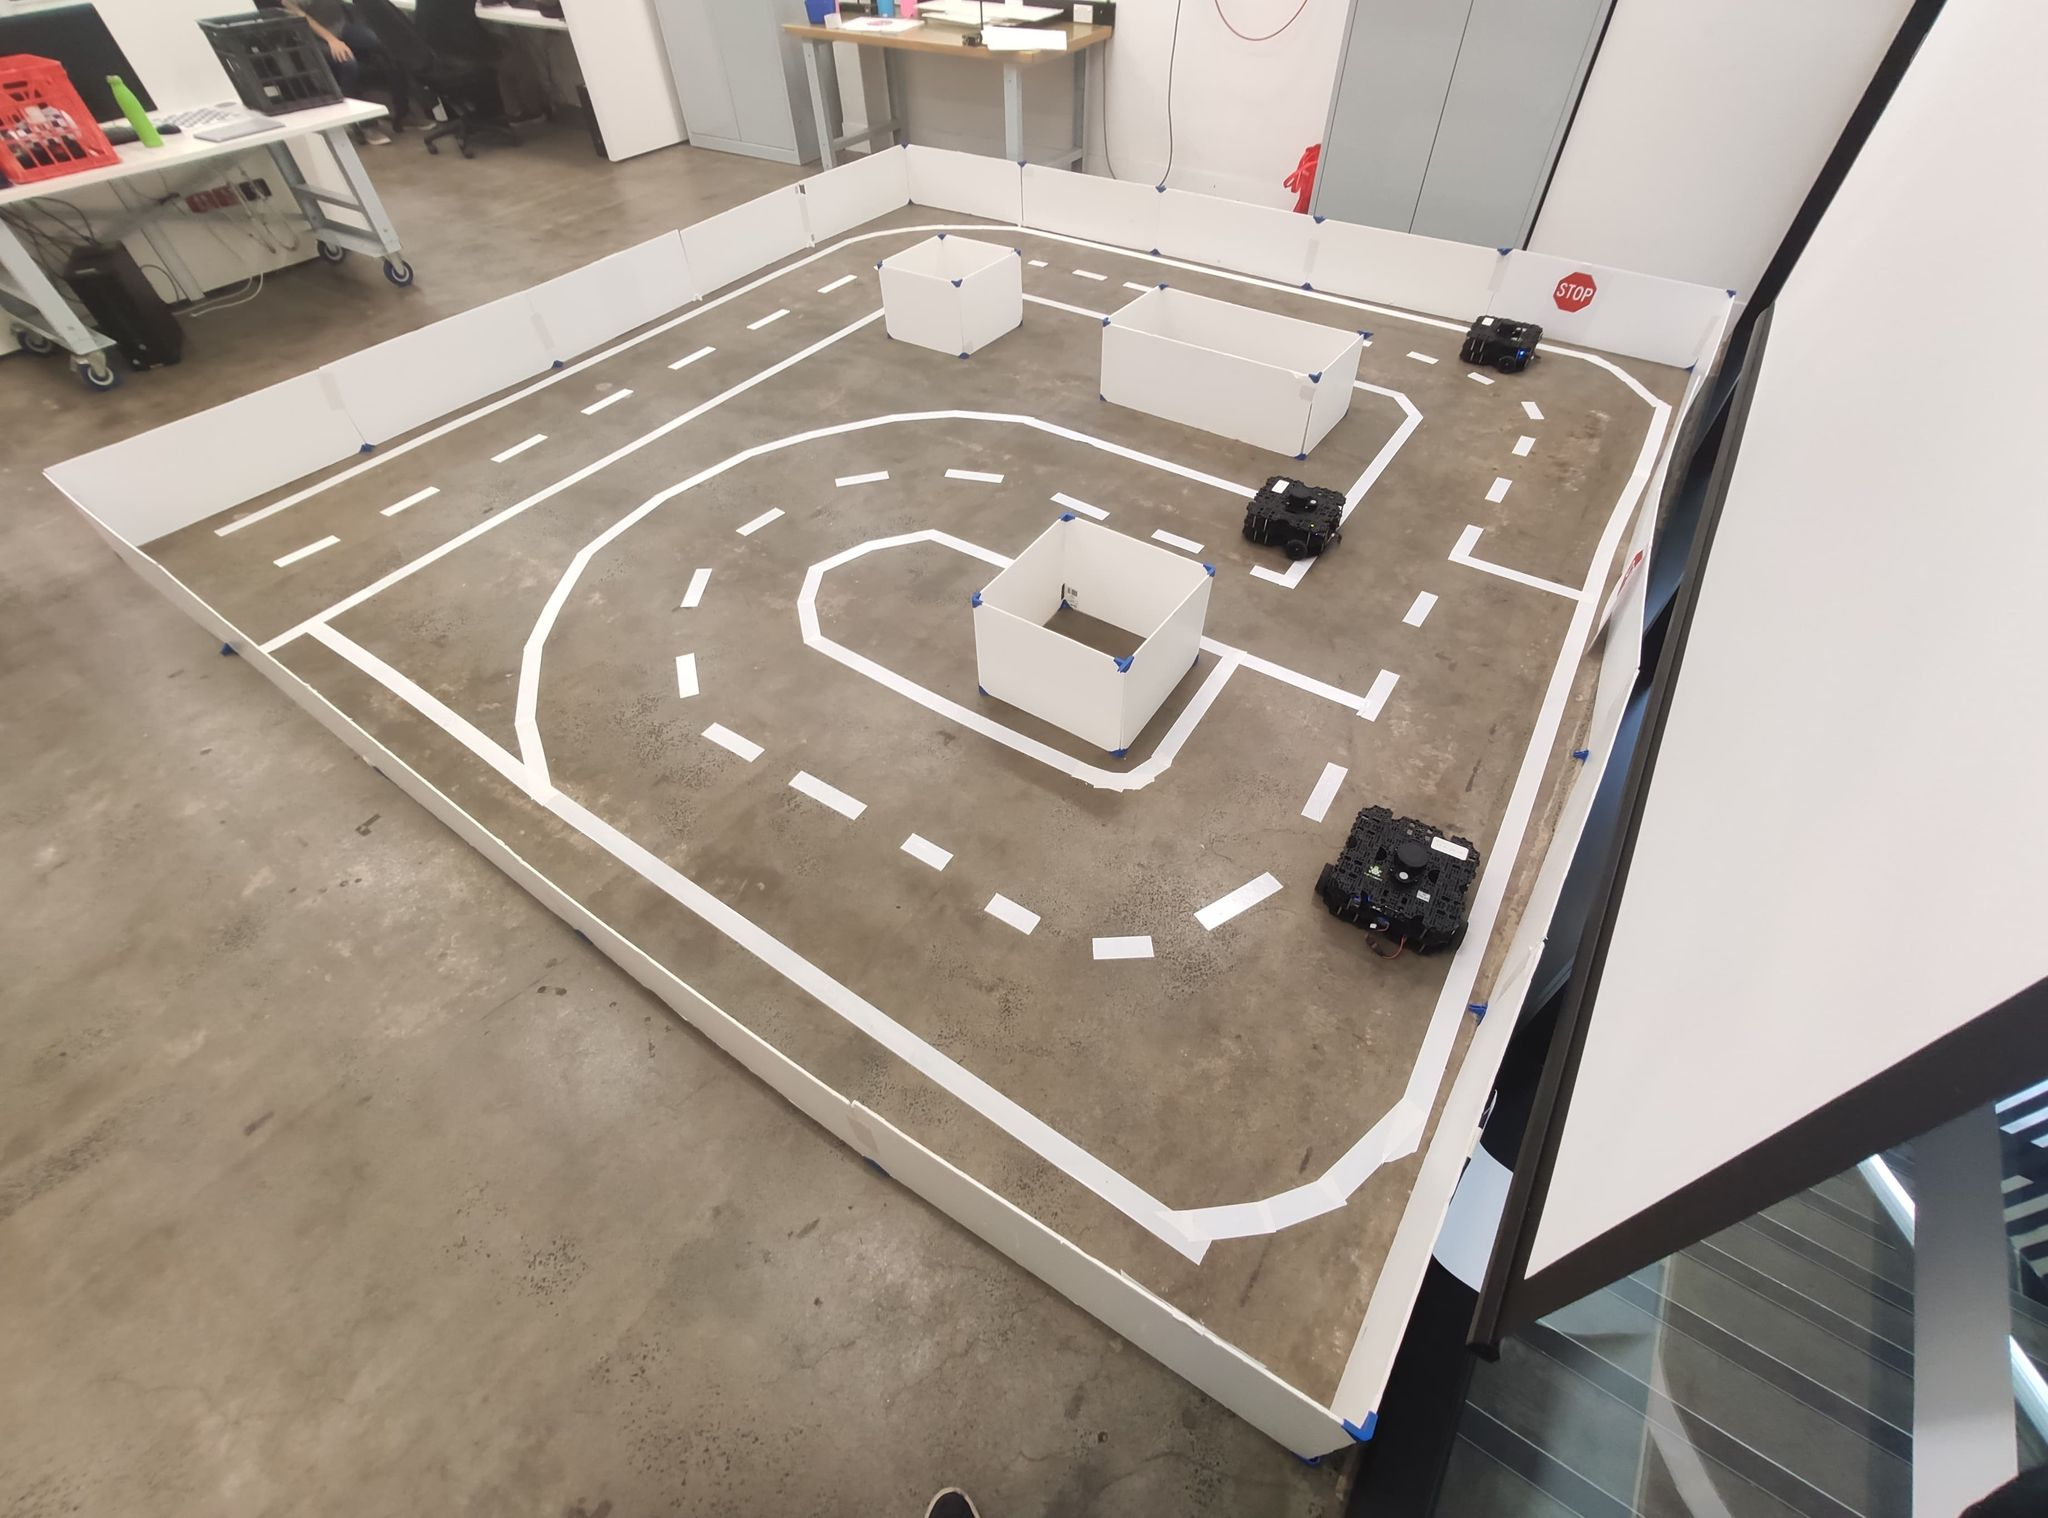
\includegraphics[width=100mm]{images/environment.jpg}
        \caption{Turtlebot Environment}
        \label{fig:environment}
    \end{figure}

    It can be assumed that there exists white walls bounding the environment, the lane markers are thick and white, stop signs are red, and turtlebots are black. It is also assumed there is constant illumination, there are no dynamic environmental changes, and road conditions are sparse and flat.

\section{Robotic Software Architecture}
\label{sec:stack}

    From the summary of the environment in Section \ref{sec:environment}, the computer vision objectives can be outlined as:
    \begin{itemize}[noitemsep, nolistsep]
        \item Lane detection
        \item Turtlebot detection
        \item Stop sign detection
    \end{itemize}

    The technologies that achieve the computer vision objectives can be abstracted as the vision processing layer of the autonomous driving stack. The output of this stack is an interpretation of the world which is inputted to a central decision-maker (robot control layer) which encapsulates a state machine representation and commands for actuation. The interactions between the world and software layers is visualised in Figure \ref{fig:stack_diagram} below.

    \begin{figure}[h!]
        \centering
        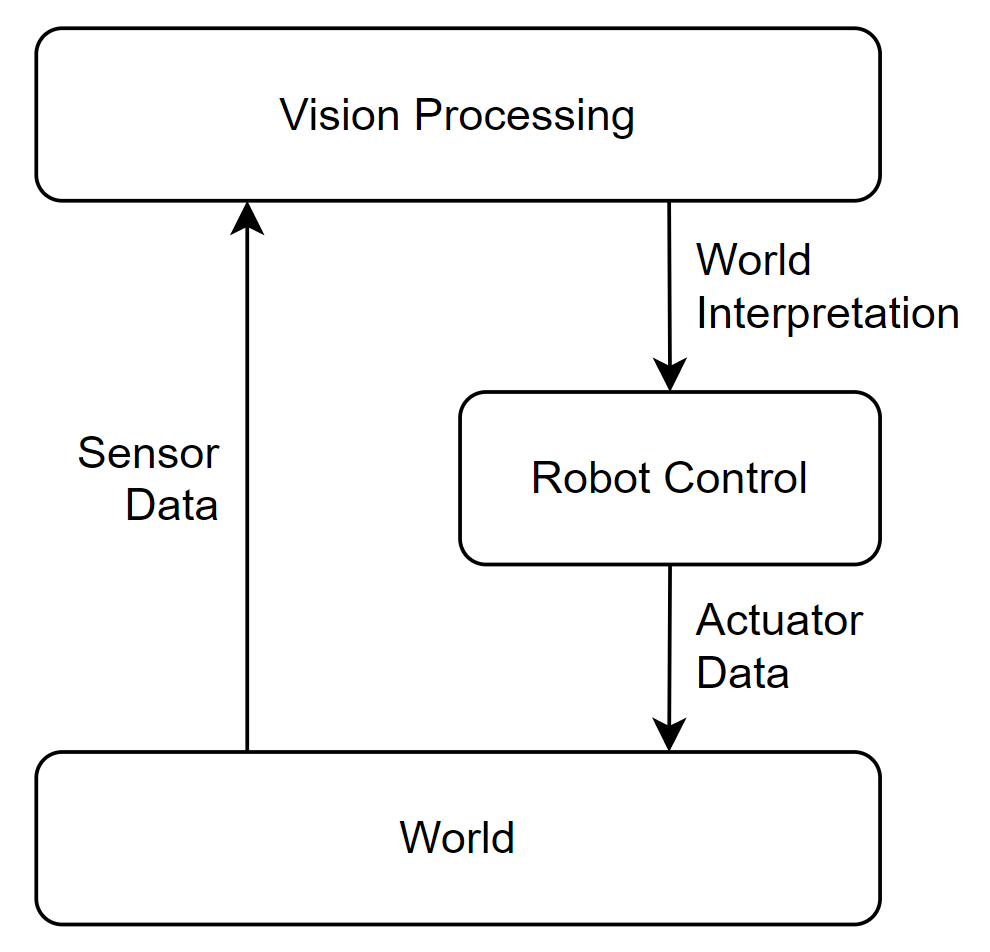
\includegraphics[width=55mm]{images/stack.png}
        \caption{Autonomous Driving Software Architecture}
        \label{fig:stack_diagram}
    \end{figure}

    The autonomous driving stack can be broken down into a publisher-subscriber pattern using ROS framework (Figure \ref{fig:ros_node_diagram} below).

    \begin{figure}[h!]
        \centering
        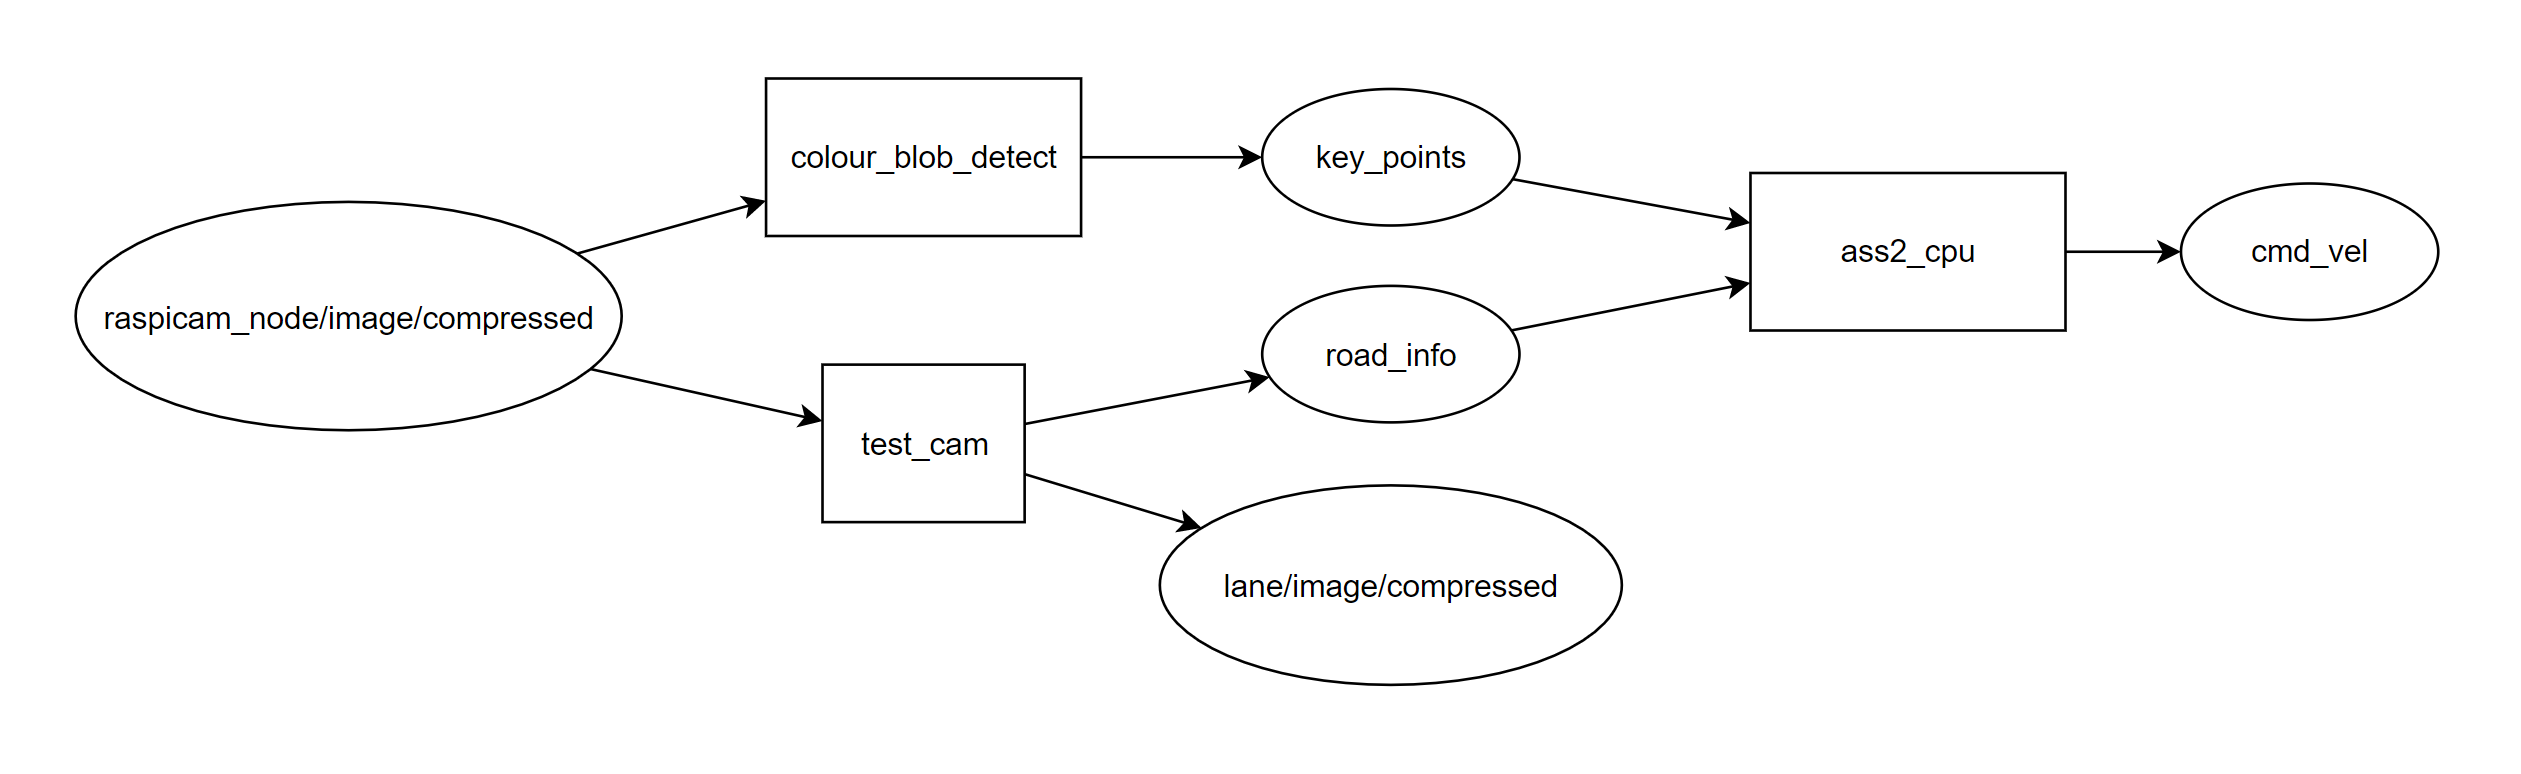
\includegraphics[width=\textwidth]{images/ros_node_diagram.png}
        \caption{Autonomous Driving ROS Node Diagram}
        \label{fig:ros_node_diagram}
    \end{figure}

    The autonomous driving stack consists of three nodes:
    \begin{itemize}[nolistsep, noitemsep]
        \item \textbf{colour\_blob\_detect}: Handles the detection of stop signs and turtlebots.
        \item \textbf{test\_cam}: Handles the detection and interpretation of lanes.
        \item \textbf{ass2\_cpu}: Encapsulates the state machine representation.
    \end{itemize}

    And consists of four fundamental topics:
    \begin{itemize}[nolistsep, noitemsep]
        \item \textbf{raspicam\_node/image/compressed}: Contains images from a Raspberry Pi camera.
        \item \textbf{key\_points}: Contains a boolean that is true for successful detection of a stop sign or turtlebot.
        \item \textbf{road\_info}: Contains lane metrics.
        \item \textbf{cmd\_vel}: Contains the velocity message to actuate the Turtlebot.
    \end{itemize}

    The lane/image/compressed topic is for visual debugging using RQT.

    \subsection{Lane Detection}

    The ROS node, ``test\_cam", subscribed to ``raspicam\_node/image/compressed" and published a custom ROS message type RoadInfo to ``road\_info". This node handled the detection and interpretation of lanes where the pseudocode is \cite{lane_metrics}:

    \begin{verbatim}
    function detectLanes(image):
        edges = get_canny_edges(image)
        edges = dilate_edges(edges)
        road_info[0] = (1 - (edges[:, 0] != 0)[::-1]).argmax()
        road_info[1] = (edges[-1] != 0).argmax()
        road_info[2] = (1 - (edges[:, 320] != 0)[::-1]).argmax()
        road_info[3] = (edges[-1] != 0)[::-1].argmax()
        road_info[4] = (1 - (edges[:, -1] != 0)[::-1]).argmax()
        return road_info
    \end{verbatim}

    RoadInfo which is of type uint32[] representing distances in the following diagram in Figure \ref{fig:road_info_diagram} below. Each integer in the diagram represents an index of the array (from 0 to 4).

    \begin{figure}[h!]
        \centering
        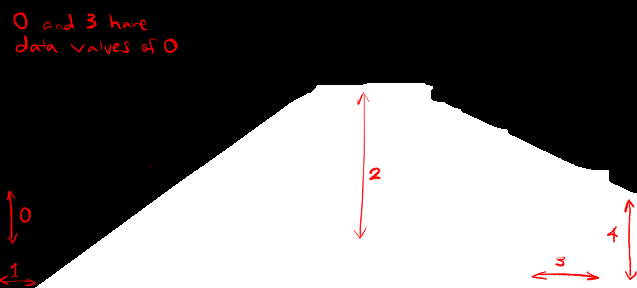
\includegraphics[width=110mm]{images/road_info.png}
        \caption{Road Information Diagram}
        \label{fig:road_info_diagram}
    \end{figure}

    Intersections are trivially detected if the lane height is large and constant in thickness, that is:

    \begin{verbatim}
    at_intersection = true if road_info[0] - road_info[4] -> 0 else false
    \end{verbatim}

    \subsection{Blob Detection}

    The ROS node, ``colour\_blob\_detect", handled the detection of both stop signs and turtlebots to simplify code complexity as the computer vision technique to detect stop signs and turtlebots were the same i.e. using OpenCV2's simple blob detector. This simple blob detector was considered for its ease of use which allowed rapid development and greater confidence in code correctness. It is also guaranteed that no other objects in the environment will be red or black other than stop signs and turtlebots respectively.
    
    The ``colour\_blob\_detect" node subscribed to ``raspicam\_node/image/compressed" and published a boolean to ``key\_points". With each subscriber callback, the obtained image was decompressed and passed into the functions: detectTurtlebot (see Appendix \ref{app:detect_turtlebot}) and detectStopSign (see Appendix \ref{app:detect_stop}). These functions followed roughly the same function structure:
    \begin{outline}[enumerate]
        \1 Apply mask to detect colour of choice.
            \2 To detect the red stop sign, the image was first converted to an HSV image which was a better colour model for masking red.
        \1 Invert the mask.
            \2 This step depends on whether the simple blob detector detects black or white blobs. It may be omitted.
        \1 Fill holes in the mask.
            \2 For detectStopSign, a morphological open then morphological close was performed on the mask to fill the ``STOP'' text.
            \2 For detectTurtlebot, a flood fill was used to fill the spaces in the turtlebot.
        \1 Get keypoints (i.e. blob coordinates and size) from applying OpenCV2's Simple Blob Detector on the mask.
        \1 Parse through the keypoints for a valid blob representation.
        \1 Return the boolean on detection of valid blob.
    \end{outline}

    \subsection{State Machine Representation}

    The robot control layer which consists of the state machine representation is encapsulated in a single node, ``ass2\_cpu". The state machine is visualised in Figure \ref{fig:state_machine} below.

    \begin{figure}[h!]
        \centering
        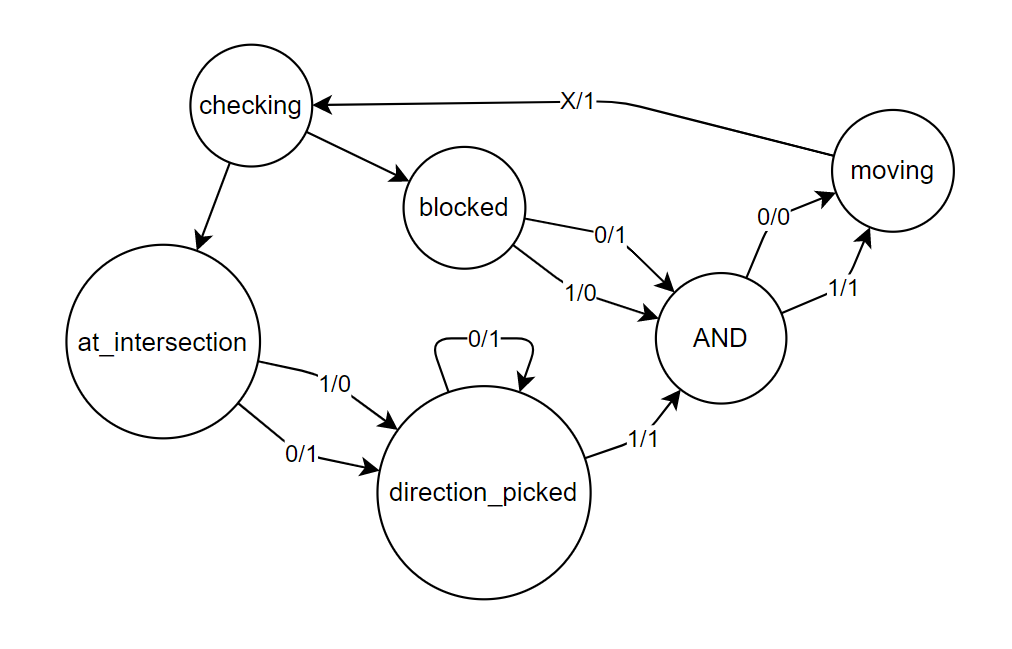
\includegraphics[width=110mm]{images/state.png}
        \caption{State Machine Representation}
        \label{fig:state_machine}
    \end{figure}

    If the boolean returned in ``colour\_blob\_detect" is true then blocked is true. If an intersection is detected then at\_intersection is true, and a suitable direction is picked to cross the intersection. If the intersection is not detected (i.e. the turtlebot is on a directed road) then the direction picked is trivial. The moving state publishes the linear and rotational velocity values to the ``cmd\_vel'' topic which is processed by the ROS navigation stack.

\section{Evaluation}
\label{sec:evaluation}

    The results of the demonstration of the autonomous driving software stack have not been released, therefore the evaluation of the autonomous driving stack can only be discussed qualitatively. The software architecture was successful in achieving autonomous driving and performed well in directed roads. Intersection handling had some difficulties causing the turtlebot to turn too early as a result of the method of detecting intersections. This could be solved by processing the stop line of the intersection instead of applying a mask over it, therefore losing visual information. The detection of stop signs and turtlebots was excellent and integrated well with the state machine intersection handler (especially in simulation). Static test results of the turtlebot and stop sign detections can be found in Appendix \ref{app:detect_turtlebot_results} and \ref{app:detect_stop_sign_results} respectively.

\section{Personal Contribution}
\label{sec:contribution}

    My contributions to this project was:
    \begin{itemize}
        \item Research into a suitable detection method of stop signs and turtlebots using the OpenCV2 library.
        \subitem \textit{OpenCV2's simple blob detector was an extremely simple and effective tool to detect stop signs and turtlebots. The detection of blobs was also a trivial problem, therefore no further research was conducted.}
        \item Design, development, and testing of ``colour\_blob\_detect" node.
        \item Integration of ``colour\_blob\_detect" with the ``ass2\_cpu" node.
    \end{itemize}

    It was difficult to incorporate my teammate's research and works involving state machine representation and lane detection as I did not work on those systems - inherent to a task allocated work-style. Therefore, this report does not offer the best detail of the other systems.

\section{Conclusion}
\label{sec:conclusion}

    Autonomous driving has clear benefits to how society travels by automobile but requires extensive research and development before the technology can be widely-commercialised. This report discussed the design of a 2-layered software architecture which was fundamental and simplistic, and covered vision processing in a high-level description. This software architecture was then verified through demonstration, where the architecture achieved autonomous driving and the computer vision objectives of lane, turtlebot, and stop sign detection.

\pagebreak

%%%%%%%%%%%%%%%%%%%%%%%%%%%%%%%%%%%%%%%%%%%%%%%%%%%%%%%%%%%%%%%%%%%%%%%%%%%%%%%%

\begin{thebibliography}{3}

    \bibitem{autonomous_driving_changes_future} Chai, Z, Nie, T \& Becker, J. 2021, Autonomous Driving Changes the Future 1st ed. 2021., Springer Singapore : Imprint: Springer, Singapore.

    \bibitem{lane_metrics} Formoso, R. 2020. Available at: \url{https://github.com/COMP3431-Bob-Ros/ass2/blob/main/ass2_test/scripts/test_cam.py}

\end{thebibliography}

%%%%%%%%%%%%%%%%%%%%%%%%%%%%%%%%%%%%%%%%%%%%%%%%%%%%%%%%%%%%%%%%%%%%%%%%%%%%%%%%

\begin{appendices}

\section{Turtlebot Detection Pseudocode}
\label{app:detect_turtlebot}

    The following pseudocode uses OpenCV2 to detect turtlebots by applying a binary mask over the black regions of the image and using simple blob detector to generate keypoints. Keypoints are parsed for a valid representation of a turtlebot and returns a boolean if a turtlebot is detected.

    \begin{verbatim}
    function detectTurtlebot(image):
        mask = apply_black_mask(image)
        mask = invert(mask)
        mask = flood_fill_holes(mask)
        keypoints = simple_blob_detector(mask, blob_params)
        detected = parseKeyPoints(keypoints, search_params)
        return detected
    \end{verbatim}

\section{Stop Sign Detection Pseudocode}
\label{app:detect_stop}

    The following pseudocode uses OpenCV2 to detect stop signs by applying a binary mask over the red regions of the image and using simple blob detector to generate keypoints. Keypoints are parsed for a valid representation of a stopsign and returns a boolean if a stopsign is detected.

    \begin{verbatim}
    function detectStopSign(image):
        image = convert_BGR_to_HSV(image)
        mask = apply_red_mask(image)
        mask = invert(mask)
        mask = morphological_open(mask)
        mask = morphological_close(mask)
        keypoints = simple_blob_detector(mask, blob_params)
        detected = parse_key_points(keypoints, search_params)
        return detected
    \end{verbatim}

\section{Turtlebot Detection Test Results}
\label{app:detect_turtlebot_results}

    Test results show the original image on the left side and the applied mask with blob circling (in red) on the right.

    \begin{figure}[h!]
        \centering
        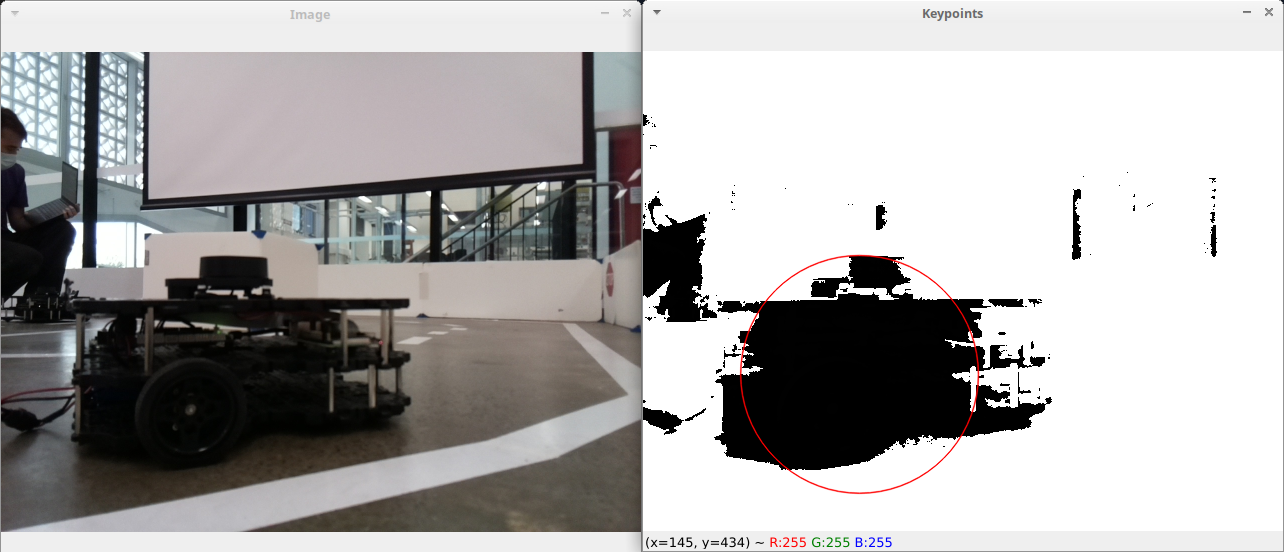
\includegraphics[width=160mm]{../test/blob/results/black_blob_1.png}
        \caption{Turtlebot Detection Test 1}
        \label{fig:turtlebot_detect_test_1}
    \end{figure}
    ~\\

    \begin{figure}[h!]
        \centering
        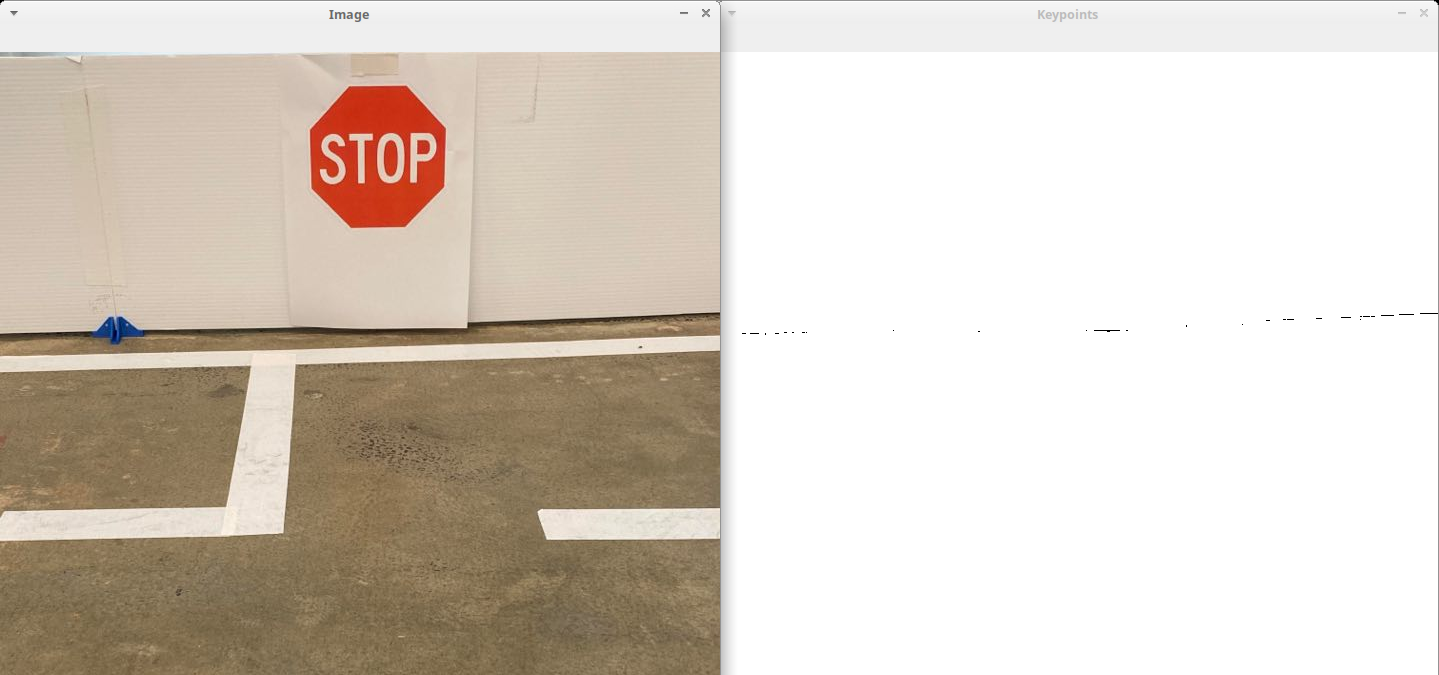
\includegraphics[width=160mm]{../test/blob/results/black_blob_2.png}
        \caption{Turtlebot Detection Test 2}
        \label{fig:turtlebot_detect_test_2}
    \end{figure}
    ~\\

    A more complex image was also tested where the mask was flood filled for stronger blob detecting.

    \begin{figure}[h!]
        \centering
        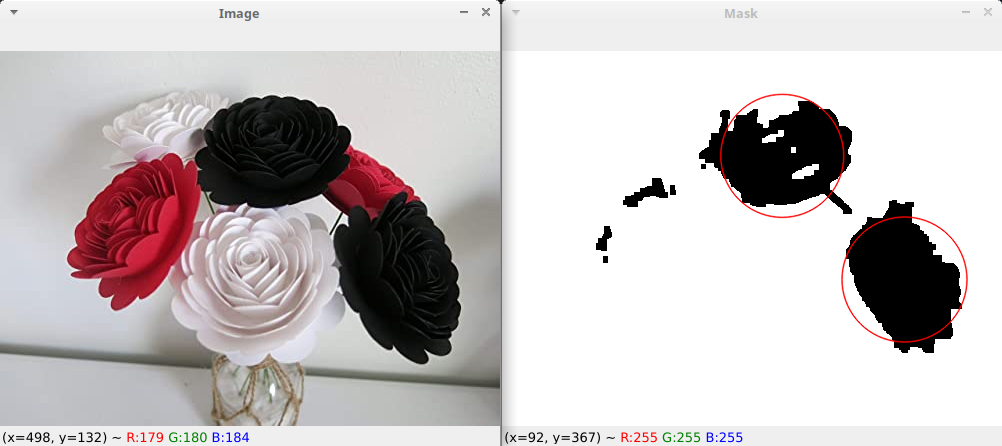
\includegraphics[width=160mm]{../test/blob/results/black_blob_3.png}
        \caption{Black Rose Detection Test}
        \label{fig:black_rose_detect_test}
    \end{figure}
    ~\\

\section{Stop Sign Detection Test Results}
\label{app:detect_stop_sign_results}

    Test results show the original image on the left side and the applied mask with blob circling (in red) on the right.

    \begin{figure}[h!]
        \centering
        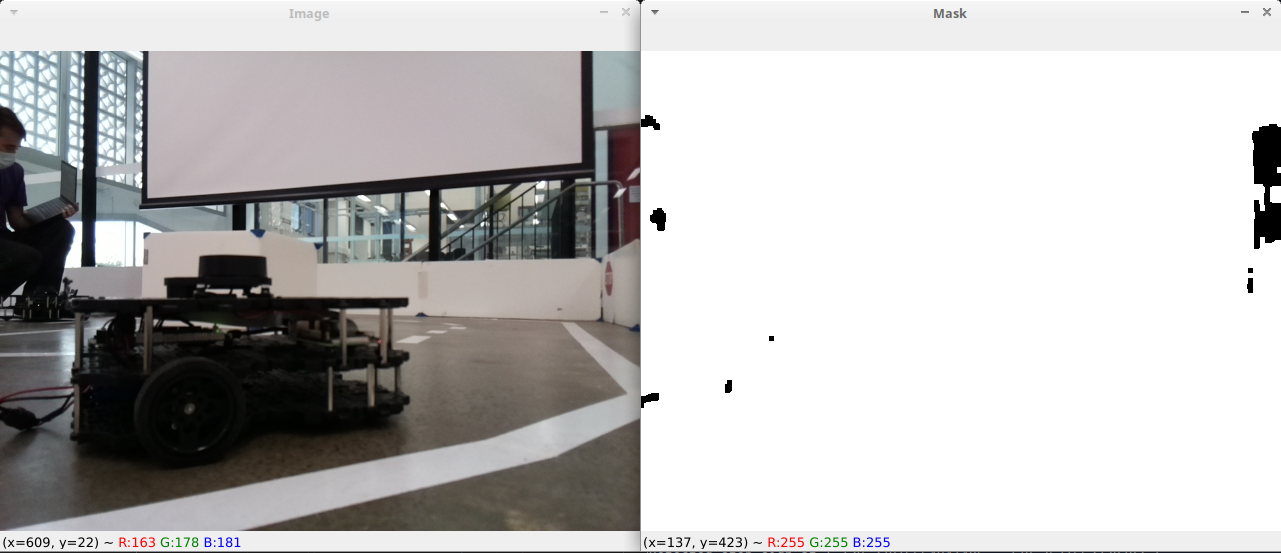
\includegraphics[width=160mm]{../test/blob/results/red_blob_1.png}
        \caption{Stop Sign Detection Test 1}
        \label{fig:stopsign_detect_test_1}
    \end{figure}
    ~\\

    \begin{figure}[h!]
        \centering
        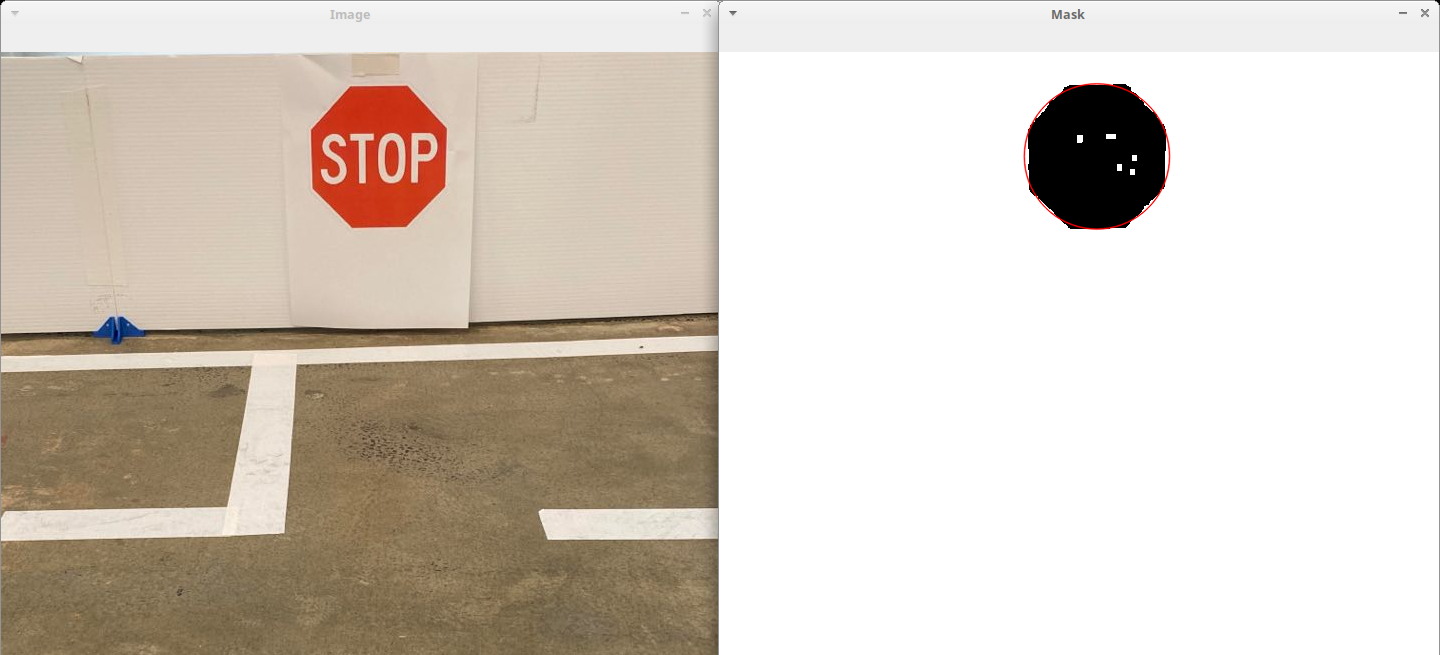
\includegraphics[width=160mm]{../test/blob/results/red_blob_2.png}
        \caption{Stop Sign Detection Test 2}
        \label{fig:stopsign_detect_test_2}
    \end{figure}
    ~\\

    A more complex image was also tested where the mask was opened then closed to fill holes for stronger blob detecting.

    \begin{figure}[h!]
        \centering
        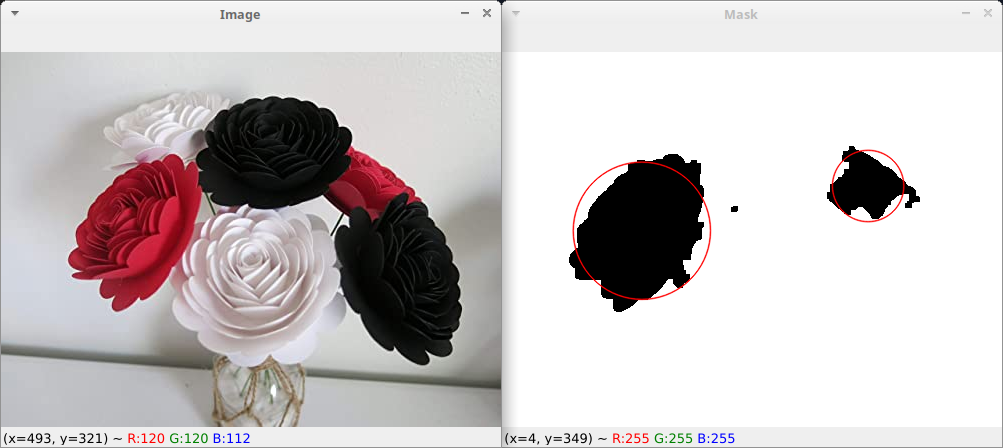
\includegraphics[width=160mm]{../test/blob/results/red_blob_4.png}
        \caption{Red Rose Detection Test}
        \label{fig:red_rose_detect_test}
    \end{figure}
    ~\\

\end{appendices}

%%%%%%%%%%%%%%%%%%%%%%%%%%%%%%%%%%%%%%%%%%%%%%%%%%%%%%%%%%%%%%%%%%%%%%%%%%%%%%%%

\end{document}